%Figure list:
% Vsum vs. traditional 2D heatmap vs. juxtaposed maps
% Chart of color bins w/r/t CIELAB threshold, with iconic maps at intervals
% Process figure
% Real examples with different color maps




\newcommand{\teaserFig}{
  \teaser{
		\centering
		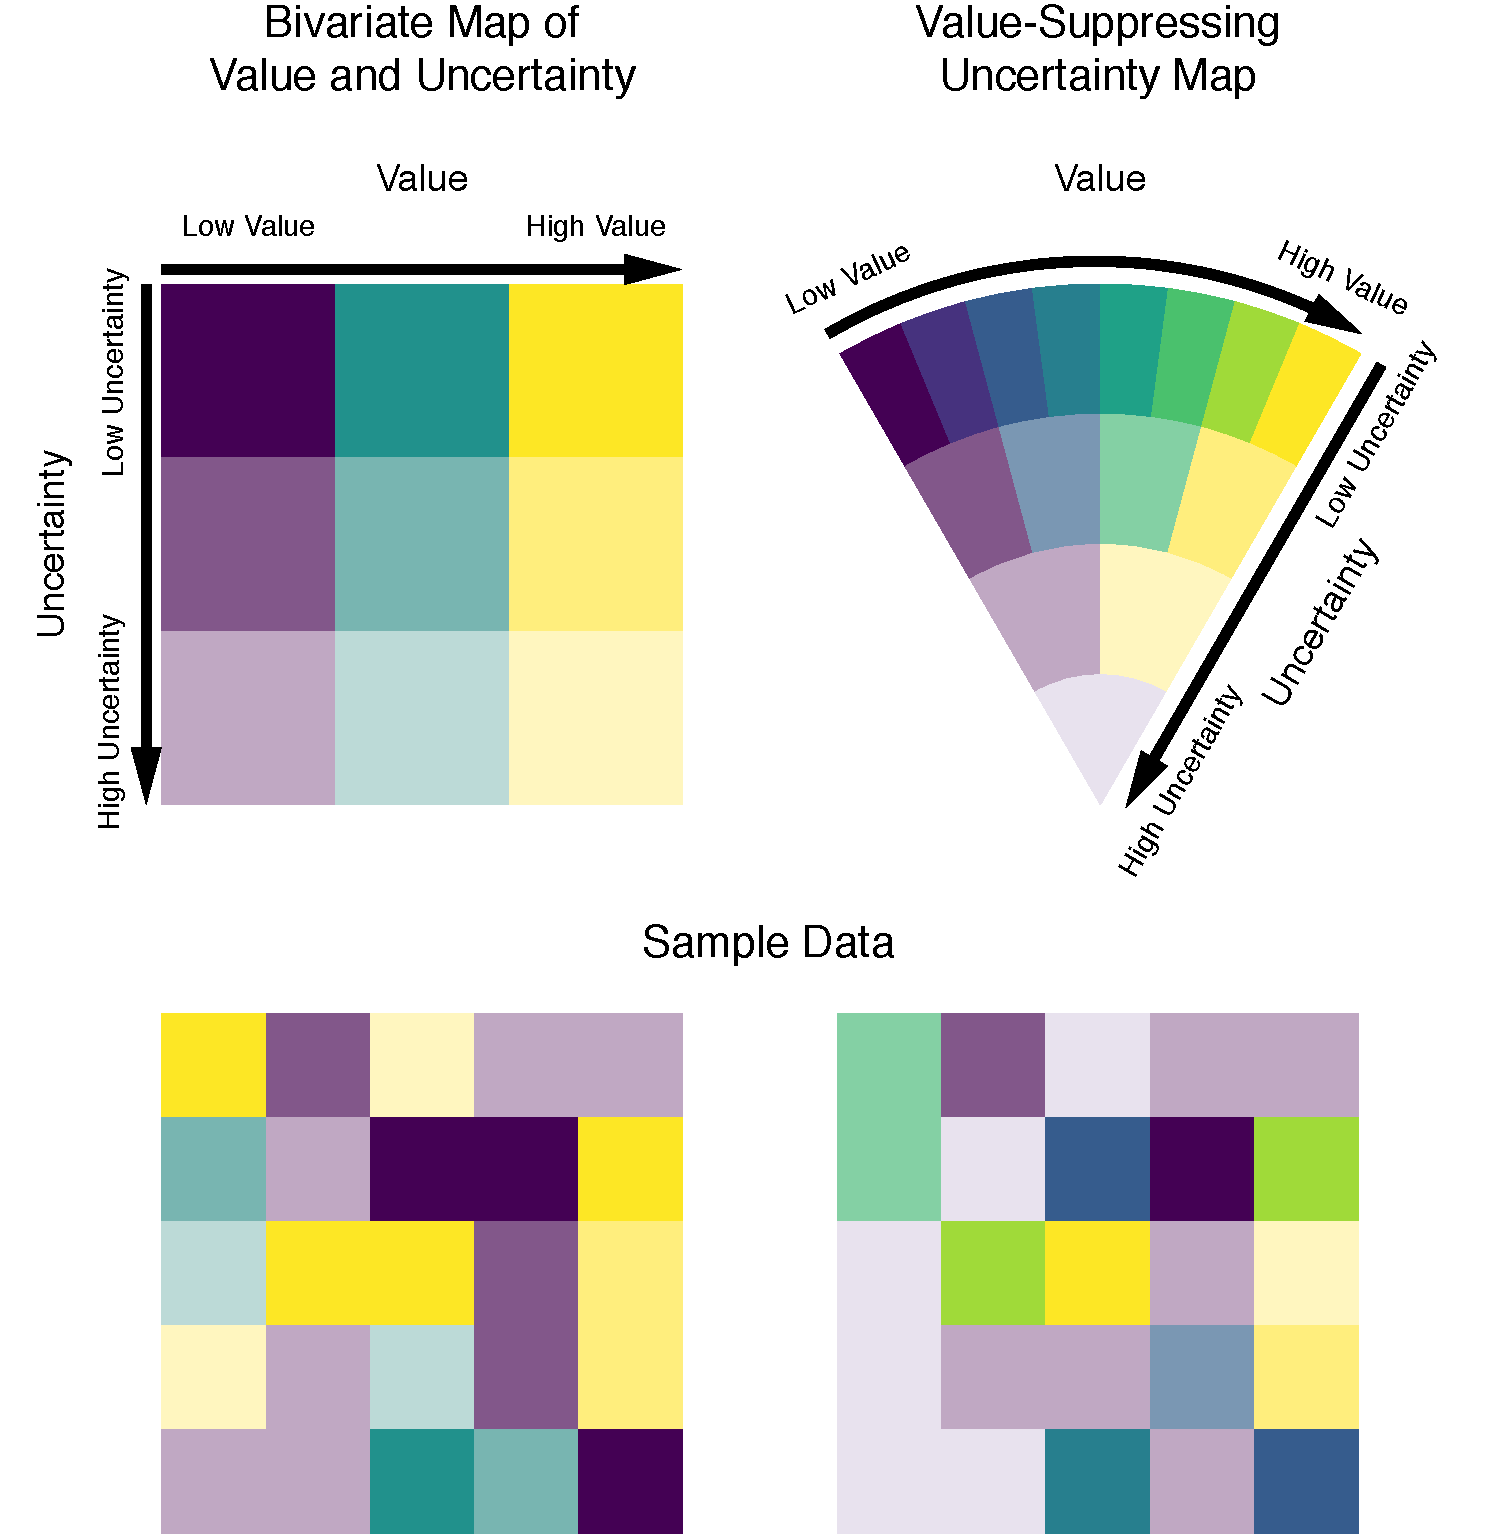
\includegraphics[width=0.9\textwidth]{example.pdf}
		\caption{Lookit! Lookit!}
		\label{fig:teaser}
	}
}

\newcommand{\exampleFig}{
\begin{figure}[t]
	\centering
	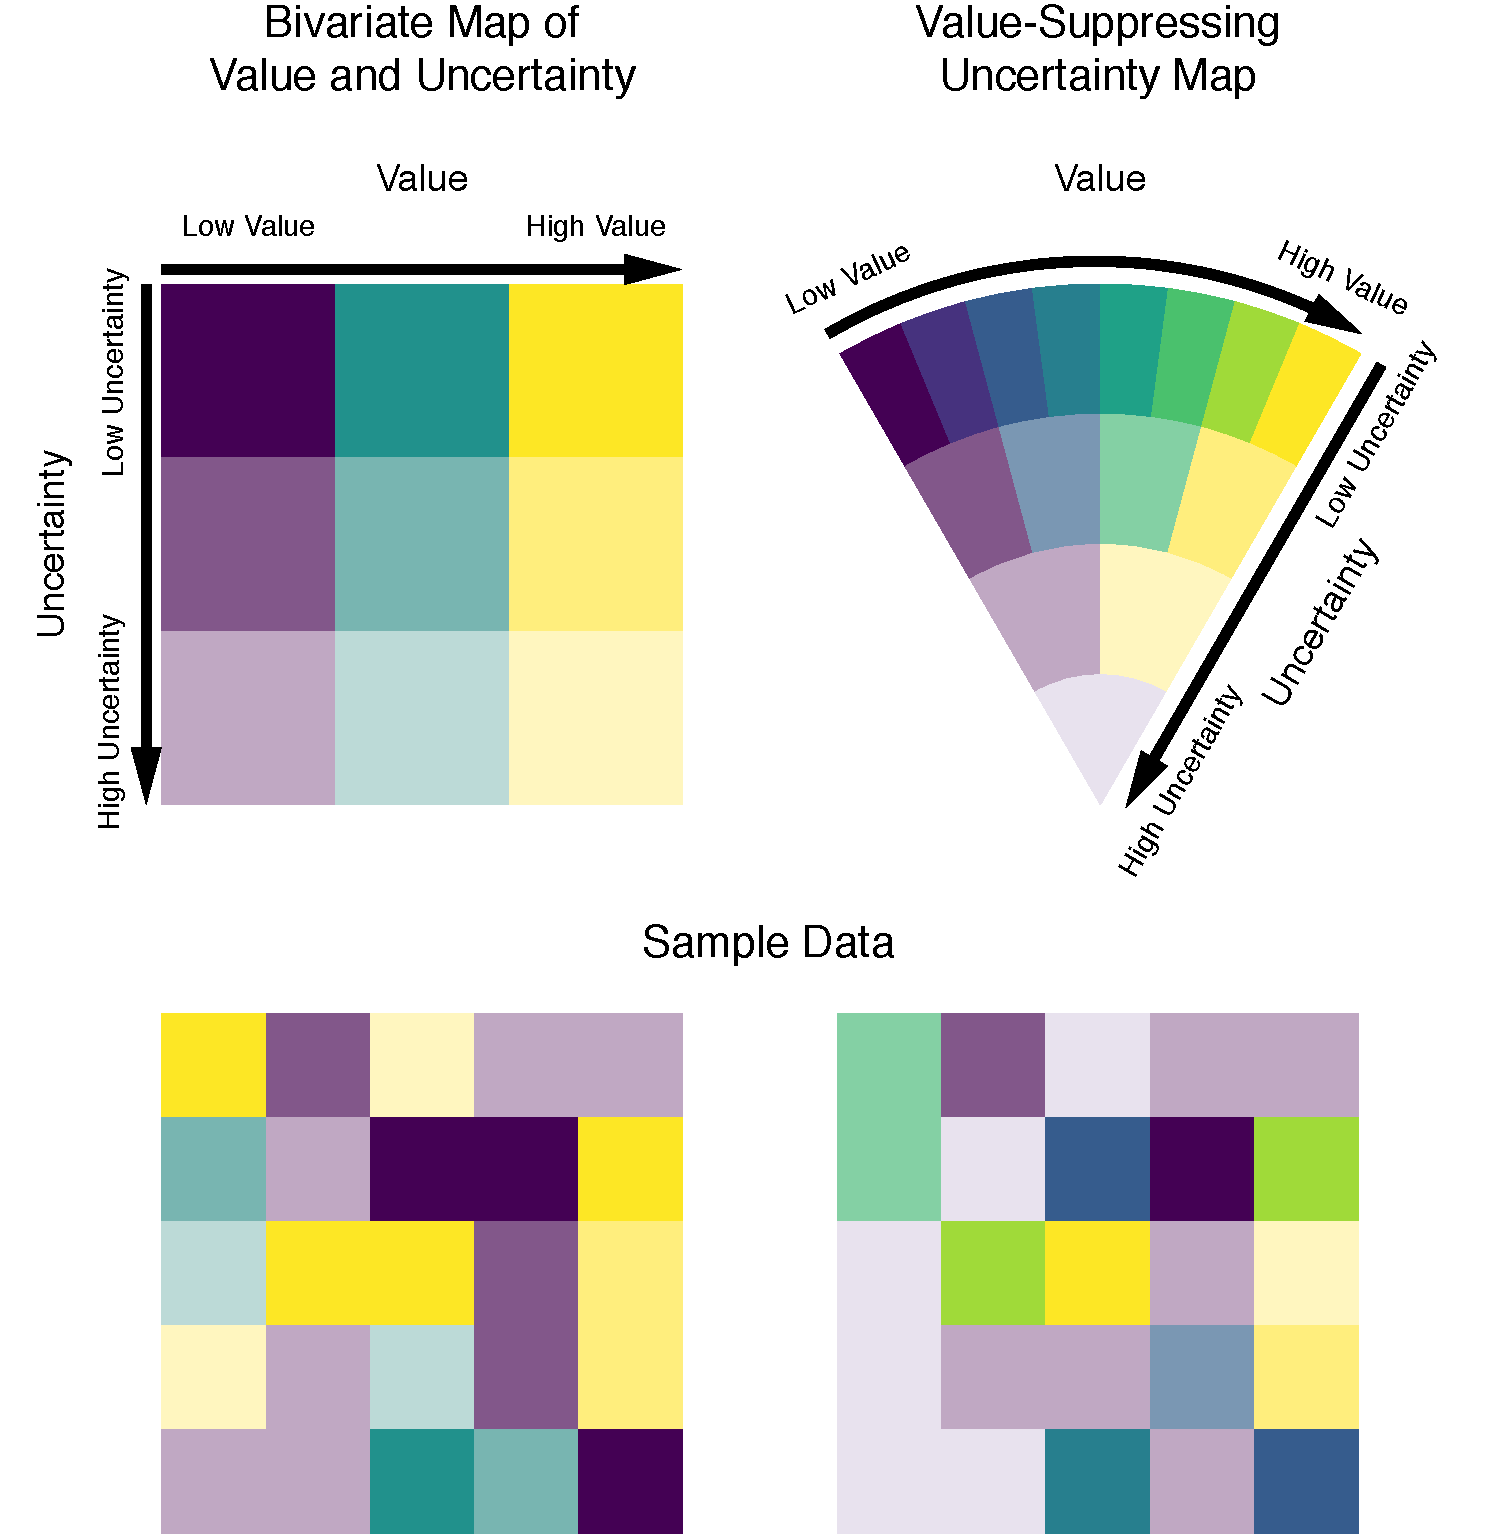
\includegraphics[width=0.9\columnwidth]{example.pdf}
	\caption{A standard bivariate map and a VSUM. Both use the same visual channels to encode value (position along the Viridis color map) and uncertainty (lightness and saturation), and have an equal standard of perceptual discriminability (at least 18 units of distance in CIELAB color space between colors). However, highly uncertain values result in colors that are very close together in the bivariate case, meaning the full bivariate map is only 9 bins under these constraints\,---\,a 4x4 map would result in colors that are perceptually too close together. By contrast, the VSUM intentionally reduces bins when uncertainty is high, eventually aliasing all highly uncertain values to the same color. This decision affords more distinct colors in other regions of the map, and so an increase in overall bins to 15. The resulting map suppresses the value of uncertain data, but increases the discriminability of data with low uncertainty.}
	\label{fig:example}
\end{figure}
}

\newcommand{\conditionFig}{
	\begin{figure*}[t]
		\centering
		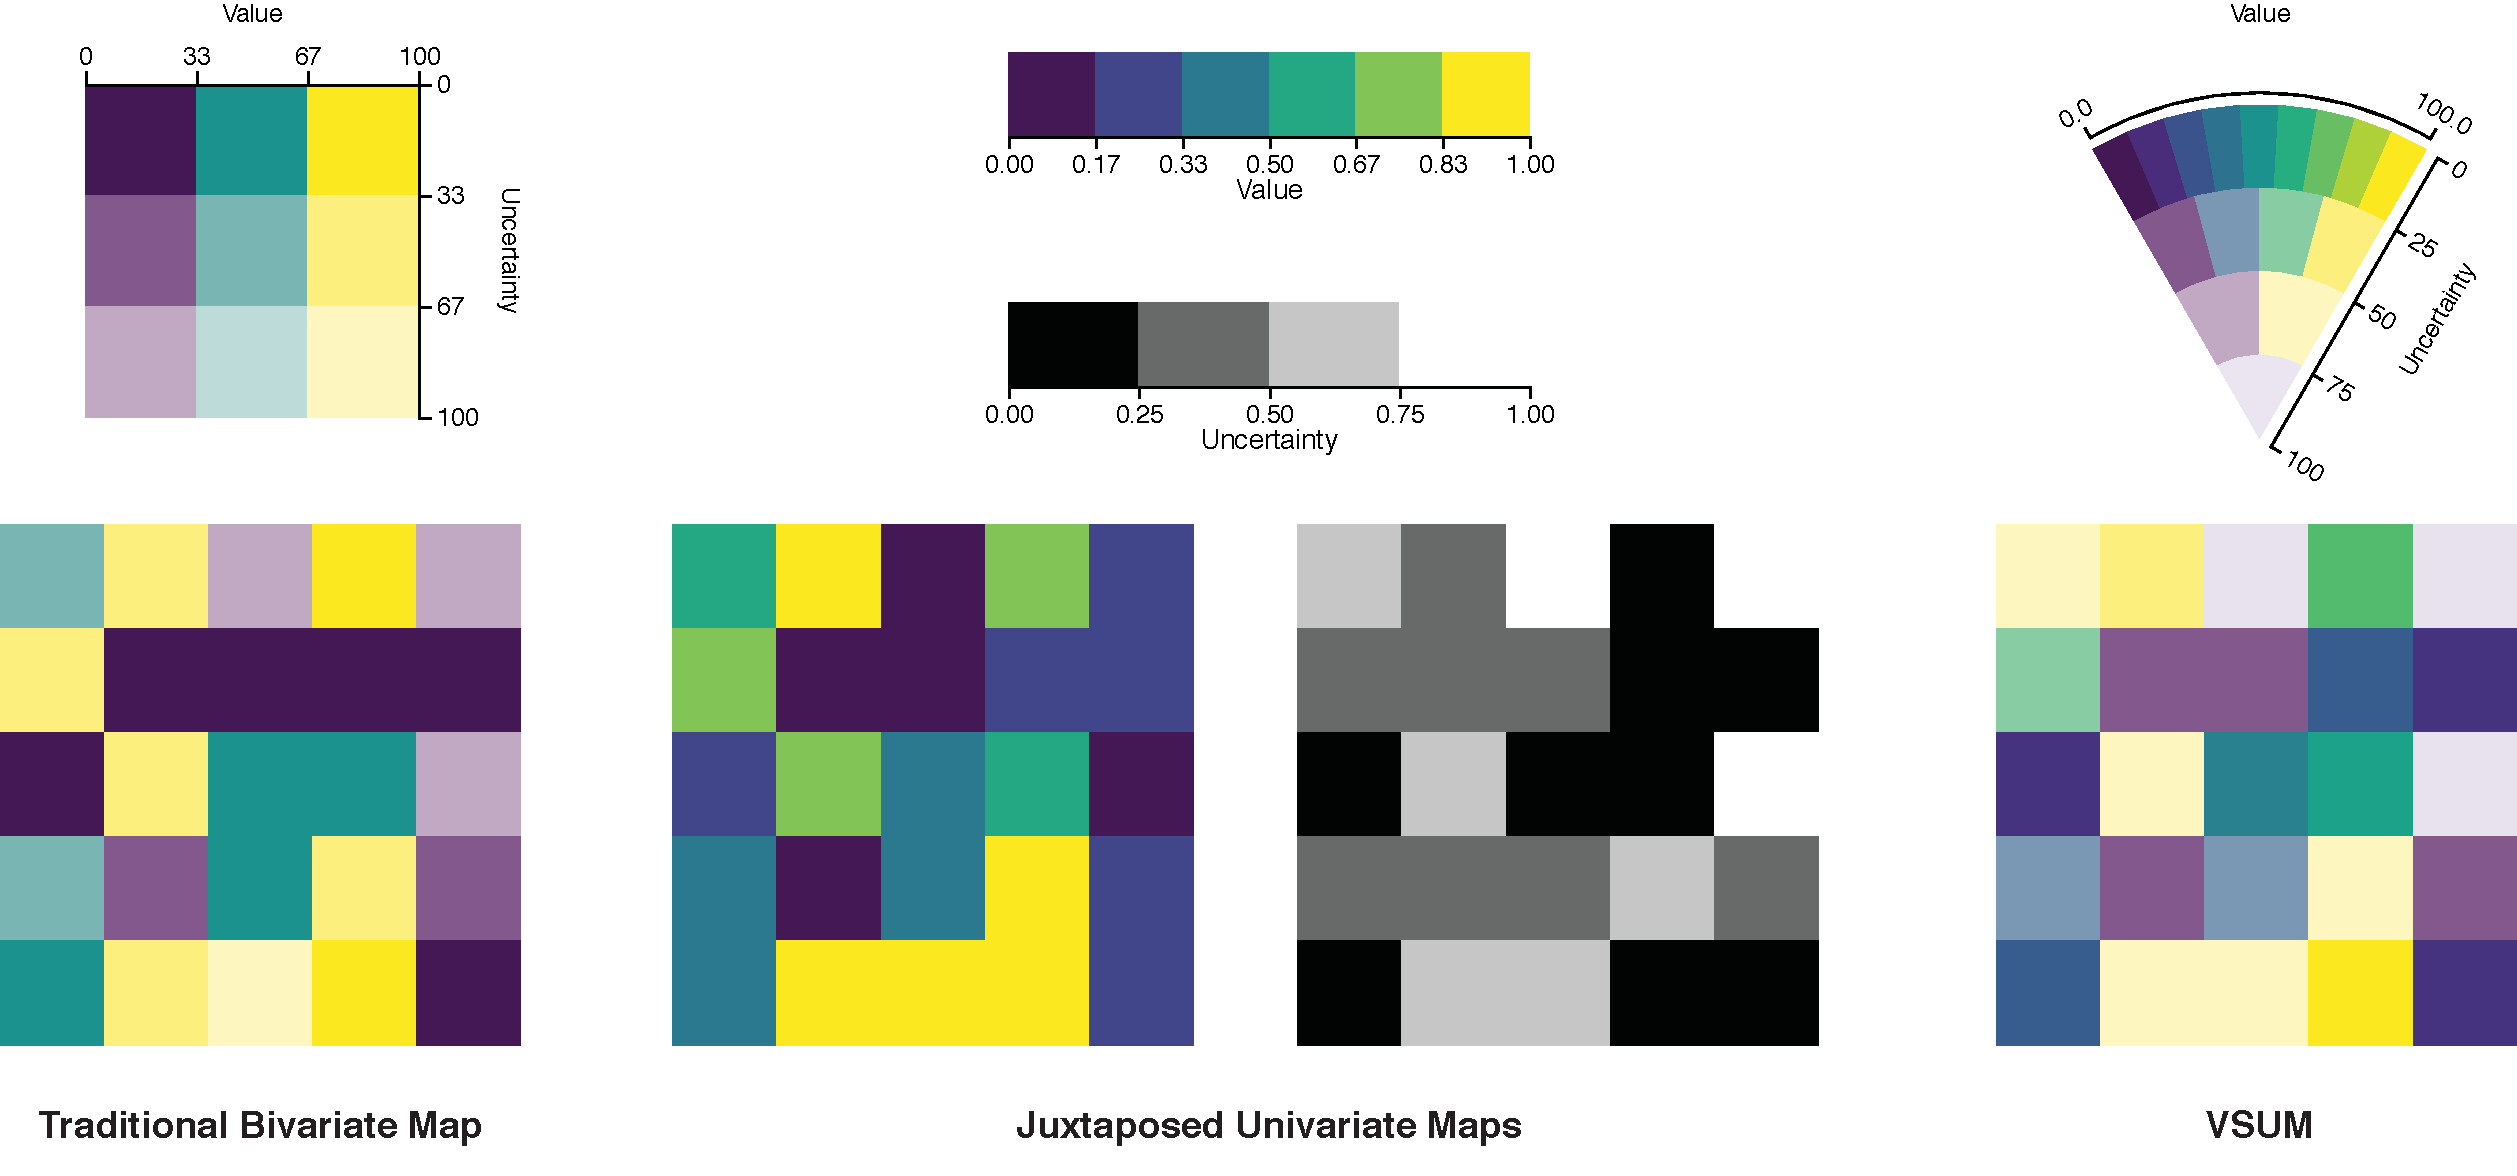
\includegraphics[width=0.8\textwidth]{conditions.pdf}
		\caption{The three graph types in our evaluation. Bivariate color ramps ensure that there are orthogonal mappings for each combination of value and uncertainty, but, since color channels are not separable, can afford only a few discrete colors before color categories become unacceptably close, perceptually. Juxtaposed maps, by keeping these channels separate, afford a larger range of colors, but require a visual search task to recover both value and uncertainty in a region. VSUMs have many of the advantages of bivariate maps, but assign more color categories to certain data, at the expense of ambiguity when uncertainty is high.}
		\label{fig:conditions}
	\end{figure*}
}

\newcommand{\taskTwoFig}{
	\begin{figure*}
		\centering
		\begin{subfigure}{0.45\textwidth}
			\includegraphics[width=\textwidth]{attack.png}
			\caption{Attacking}
			\label{fig:taskTwoAttack}
		\end{subfigure}
		~
		\begin{subfigure}{0.45\textwidth}
			\includegraphics[width=\textwidth]{defend.png}
			\caption{Defending}
			\label{fig:taskTwoDefend}
		\end{subfigure}
		\caption{The two framings of the Prediction task. In the ``attack'' framing, the participant is given a map of predictions of the location of enemy ships, along with the uncertainty in those predictions. The participant should place their missile strikes on locations with a high probability of containing a ship, and with high certainty in this probability. The ``defend'' framing is the opposite task: the participant has a list of likely missile locations, and ought to place their ships one locations with low probability of attack, and high certainty in this probability.}
		\label{fig:taskTwoConditions}
	\end{figure*}
}

\newcommand{\performanceFig}{
	\begin{figure}[t]
		\centering
		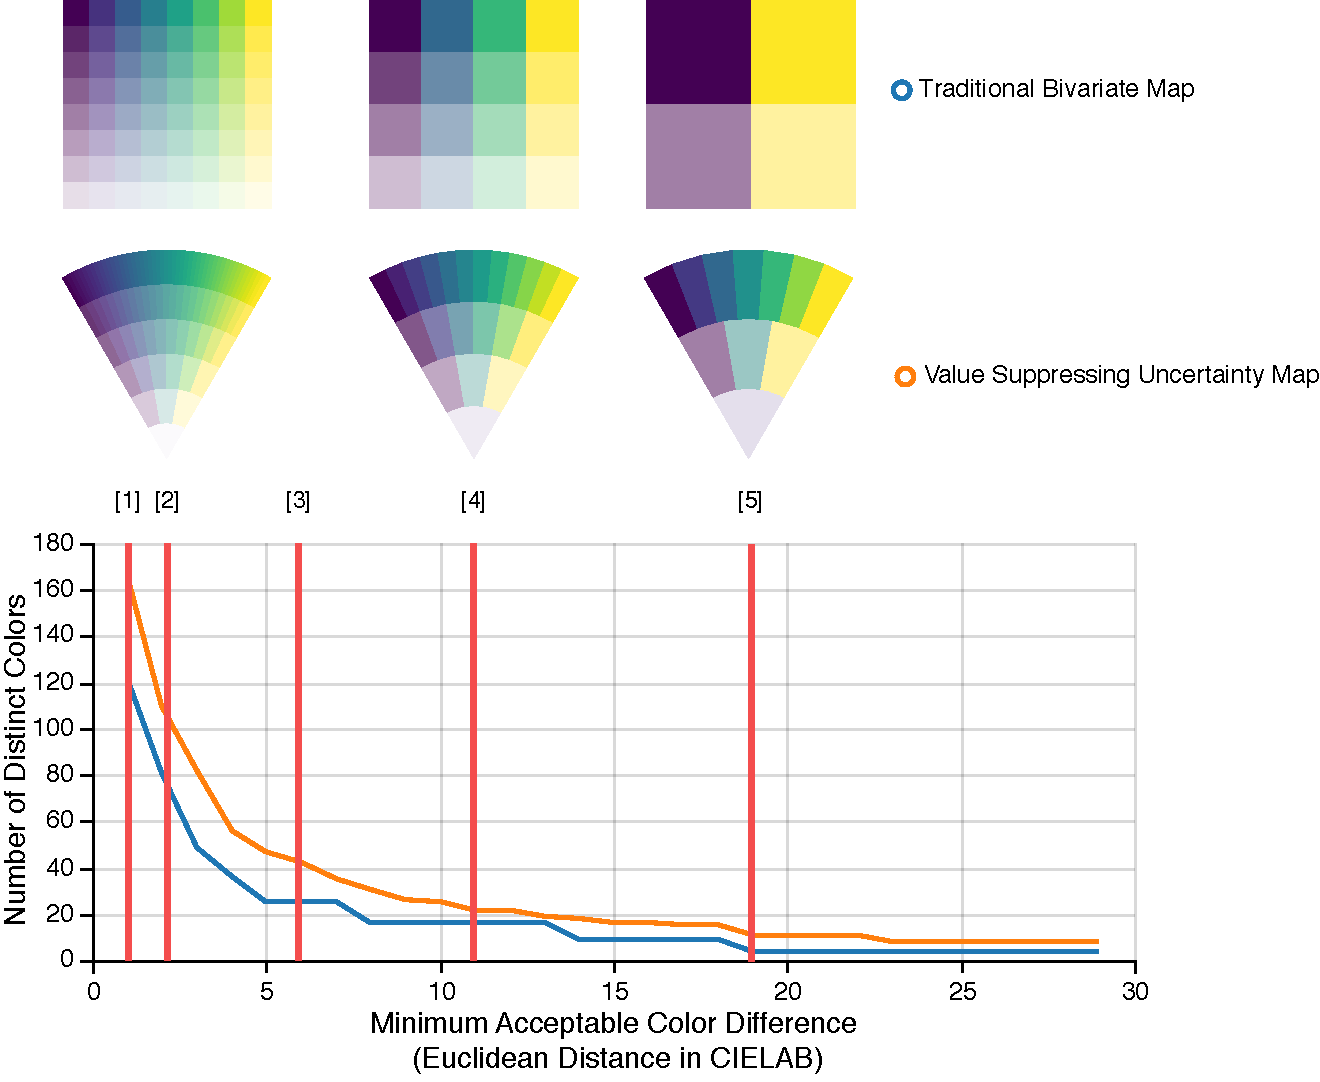
\includegraphics[width=0.9\columnwidth]{performance.pdf}
		\caption{
			The number of discrete color categories in traditional bivariate color maps versus VSUMs, assuming value is encoded by the Viridis color map~\protect\cite{garnier2015viridis}, and uncertainty is encoded by saturation/value (whiter values are more uncertain). Since these whiter uncertain colors are closer together in CIELAB space, and VSUMs intentionally require fewer color bins in those regions, VSUMs always have more color categories than the corresponding 2D bivariate map. The red lines denote:
		  \textbf{1)} Theoretical 50\% JND from CIELAB specification.
			\textbf{2)} 50\% JND from controlled lab study of Mahy et al.~\protect\cite{mahy1994evaluation}.
			\textbf{3)} 50\% JND from Szafir et al.\protect\cite{szafir2014adapting}.
			\textbf{4)} 50\% JND for small visual targets from Stone et al.~\protect\cite{stone2014engineering}.
			\textbf{5)} The threshold resulting in the simplest possible (2x2) bivariate map.
	    }
		\label{fig:performance}
	\end{figure}
}

\newcommand{\flowFig}{
	\begin{figure}[t]
		\centering
		\includegraphics[width=0.95\columnwidth]{flow.pdf}
		\caption{}
		\label{fig:flow}
	\end{figure}
}

\newcommand{\airlineFig}{
\begin{figure}[t]
	\centering
	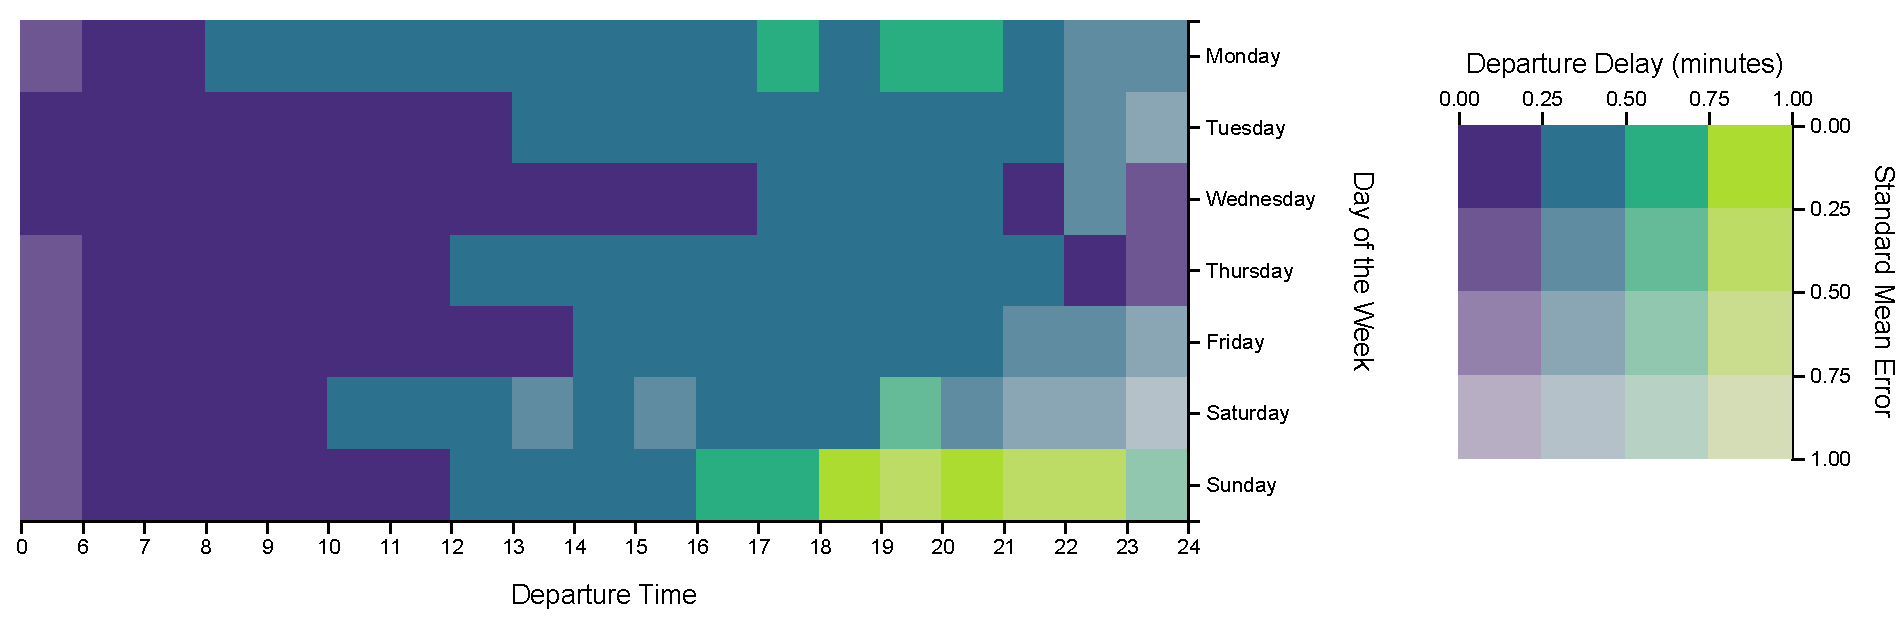
\includegraphics[width=\columnwidth]{airline-2d.png}
	\vspace{-20px}
	\caption{Average departure delay for different times of the day and days of the week visualized with a 2D uncertainty map.}
	\label{fig:airline2d}

	\vspace{10px}

	\centering
	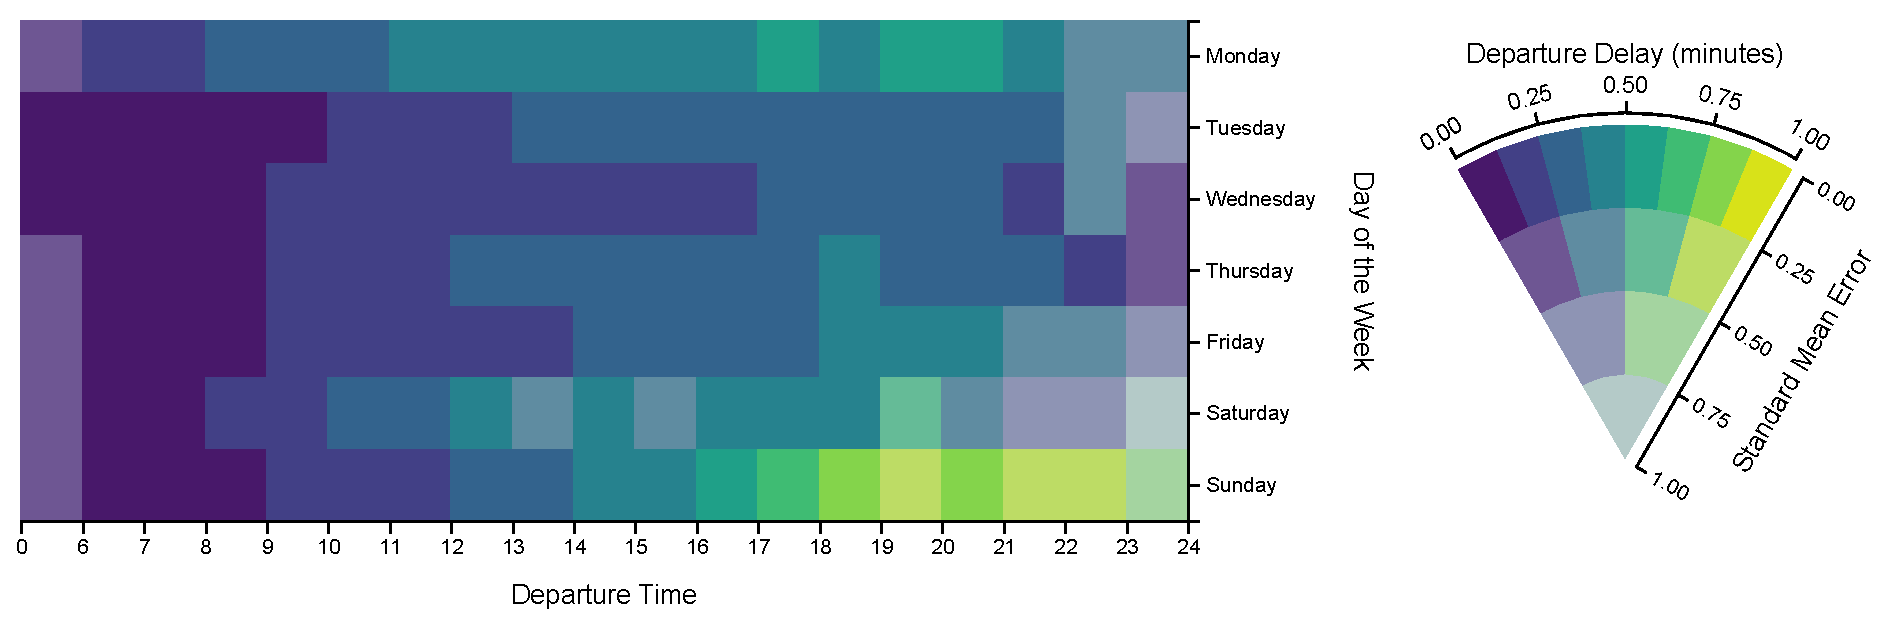
\includegraphics[width=\columnwidth]{airline-vsum.png}
	\vspace{-20px}
	\caption{Flight delay data encoded with a VSUM.}
	\label{fig:airlineVsum}
\end{figure}
}

\newcommand{\viralFig}{
\begin{figure}[t]
	\centering
	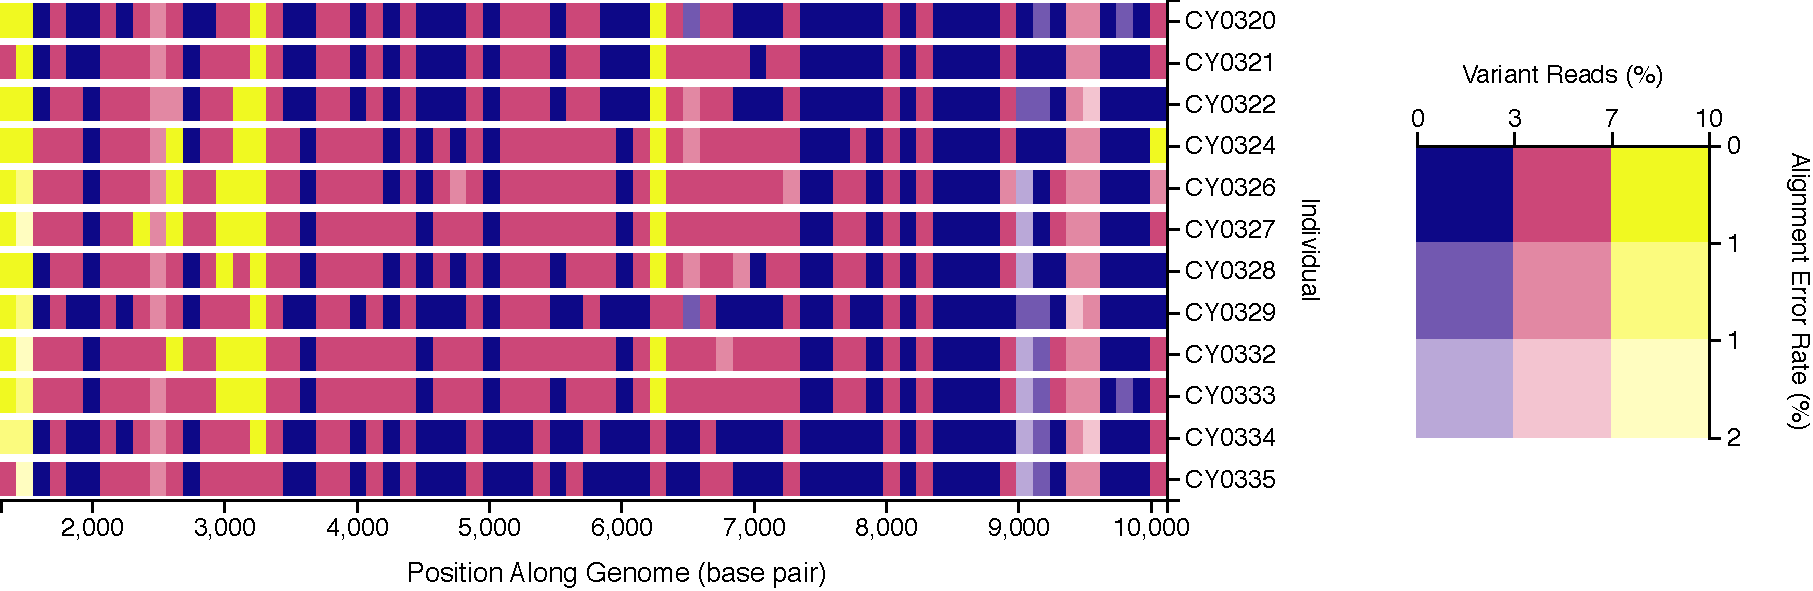
\includegraphics[width=\columnwidth]{viral-2d.pdf}
	\vspace{-20px}
	\caption{Virus genome data for reads between position $1309$ and $10124$ visualized with a 2D uncertainty map.}
	\label{fig:viral2d}

	\centering
	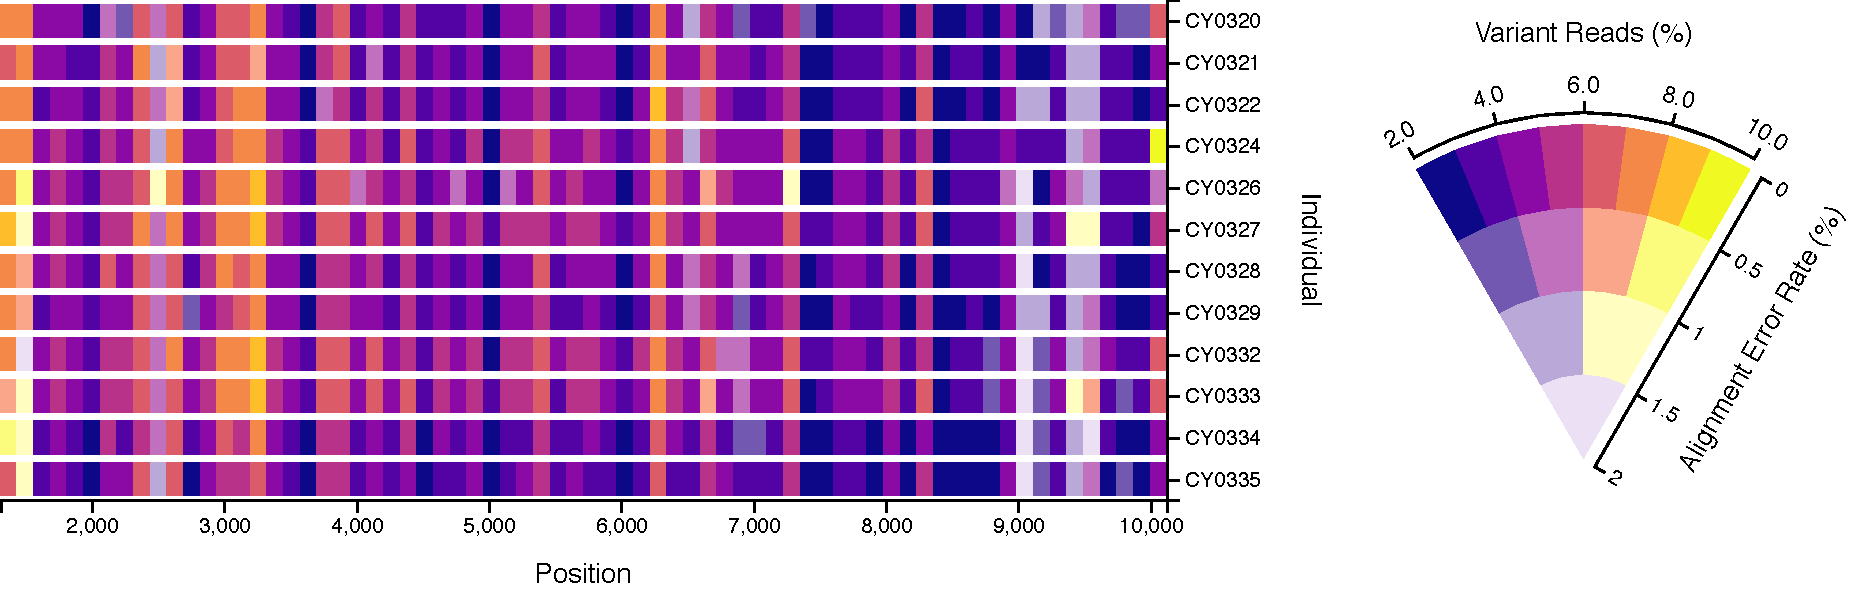
\includegraphics[width=\columnwidth]{viral-vsum.pdf}
	\vspace{-20px}
	\caption{Virus genome mutations and read error encoded with a VSUM.}
	\label{fig:viralVsum}
\end{figure}
}
